% ==================================================================
%  徐森林、薛春华《数学分析》（第二册）
%  第 10 章  $n$ 元函数的 Riemann 积分
%  §10.2  $\mathbb{R}^2$ 中有界集合上的二重积分
%  源：印刷页 199–207 (PDF p. 205–213)
% ==================================================================

\makeatletter
\newenvironment{definitionpp}{%
  \par\addvspace{1.0\baselineskip}%
  \addtocounter{definition}{-1}%
  \def\thedefinition{\thesection.\arabic{definition}\ensuremath{^{\prime\prime}}}%
  \definition
}{%
  \enddefinition
  \addvspace{1.0\baselineskip}%
}
\makeatother

\section{\texorpdfstring{$\mathbb{R}^2$}{R²} 中有界集合上的二重积分}\label{sec:10.2}

上节在 $\mathbb{R}^2$ 中的闭区间上引进了二重 Riemann 积分, 它与 $\mathbb{R}^1$ 中闭区间 $[a,b]$ 上的 Riemann 积分完全类似. 现在来定义 $\mathbb{R}^2$ 中有界集合上的 Riemann 积分.

\begin{definition}\label{def:10.2.1}
设 $\Omega \subset \mathbb{R}^2$ 为有界集, $f\colon \Omega \to \mathbb{R}$ 为二元函数. 记
\[
f_{\Omega}(\boldsymbol{x}) = f_{\Omega}(x,y) = \begin{cases}
f(x,y), & \boldsymbol{x}=(x,y)\in\Omega, \\
0, & \boldsymbol{x}=(x,y)\notin\Omega,
\end{cases}
\]
并称之为 $f$ 的零延拓. 任取闭区间 $I \supset \Omega$. 如果 $f_{\Omega}$ 在 $I$ 上 Riemann 可积, 则称 $f$ 在 $\Omega$ 上 Riemann 可积 (简称可积), 称 $\int_I f_{\Omega}$ 为 $f$ 在 $\Omega$ 上的 Riemann 积分, 记为
\[
\iint_{\Omega}f(x,y)\,\mathrm{d}x\mathrm{d}y = \int_{\Omega}f\,\mathrm{d}V = \int_{\Omega}f = \int_{\Omega}f_{\Omega} = \iint_{I}f_{\Omega}(x,y)\,\mathrm{d}x\mathrm{d}y.
\]
\end{definition}

\begin{lemma}\label{lem:10.2.1}
定义 \ref{def:10.2.1} 中 $\int_{\Omega} f$ 与包含 $\Omega$ 的闭区间 $I$ 的选取无关 $($定义的合理性$)$.
\end{lemma}

\begin{proof}
设 $I_1, I_2$ 为包含 $\Omega$ 的任两闭区间, 则 $I = I_1 \cap I_2$ 也是包含 $\Omega$ 的闭区间 (图 \ref{fig:10.2.1}). 由 $f_{\Omega}$ 的定义知 $f_{\Omega}|_{I_i \setminus I} = 0$. 再由闭区间上积分的定义得到
\[
f_{\Omega} \text{ 在 } I_i \text{ 上可积} \iff f_{\Omega} \text{ 在 } I \text{ 上可积},
\]
且
\[
\int_{I_i}f_{\Omega} = \int_I f_{\Omega}, \quad i=1,2.
\]
从而
\[
\int_{I_1}f_{\Omega} = \int_{I_2}f_{\Omega}. \qedhere
\]
\end{proof}

\begin{figure}[htbp]
\centering
\begin{tikzpicture}[scale=0.95, >=Stealth]
  % I1 矩形: (0, 0.5) 到 (3.2, 3.2)
  % I2 矩形: (1.2, -0.5) 到 (4.8, 2.2)
  % 交集 I: (1.2, 0.5) 到 (3.2, 2.2)
  \fill[gray!20] (1.2, 0.5) rectangle (3.2, 2.2);
  
  % 区域 Omega 在 I 内部
  \begin{scope}
    \clip (2.2, 1.35) ellipse [x radius=0.75, y radius=0.55, rotate=25];
    \fill[pattern=north east lines, pattern color=black!70] (1.2, 0.5) rectangle (3.2, 2.2);
  \end{scope}
  \draw[thick] (2.2, 1.35) ellipse [x radius=0.75, y radius=0.55, rotate=25];
  \node at (2.2, 1.35) {$\Omega$};
  
  % 矩形线框
  \draw[thick] (0, 0.5) rectangle (3.2, 3.2);
  \draw[thick] (1.2, -0.5) rectangle (4.8, 2.2);
  
  % 标注
  \node[below right] at (0.05, 3.1) {$I_1$};
  \node[above left] at (4.75, -0.45) {$I_2$};
  \node[above] at (2.2, 0.55) {\small $I = I_1 \cap I_2$};
\end{tikzpicture}
\caption{}
\label{fig:10.2.1}
\end{figure}

\begin{theorem}[可积的充分条件]\label{thm:10.2.1}
设 $\Omega \subset \mathbb{R}^2$ 为有界集, 函数 $f\colon \Omega \to \mathbb{R}$ 有界. 如果 $\partial\Omega$ 与 $f$ 在 $\Omega$ 上的不连续点集 $D_{\text{不}}^f$ 都为零测集, 则 $f$ 在 $\Omega$ 上可积.
\end{theorem}

\begin{proof}
取闭区间 $I$ 满足 $I^\circ \supset \overline{\Omega}$. 由于 $f_{\Omega}$ 在开集 $(\overline{\Omega})^c$ 上处处为零, 所以 $(\overline{\Omega})^c$ 上的每一点都是 $f_{\Omega}$ 的连续点. 在 $\Omega^\circ$ 上, $f_{\Omega}=f$, 所以在 $\Omega^\circ$ 上, $f_{\Omega}$ 的不连续点即为 $f$ 的不连续点. 因此, 有
\[
D_{\text{不}}^{f_{\Omega}} \subset D_{\text{不}}^f \cup \partial\Omega.
\]
由于 $D_{\text{不}}^f$ 与 $\partial\Omega$ 都为零测集, 故 $D_{\text{不}}^{f_{\Omega}}$ 也为零测集, 根据定理 \ref{thm:10.1.7}(8) 知, $f_{\Omega}$ 在 $I$ 上是可积的, 从而 $f$ 在 $\Omega$ 上是可积的.
\end{proof}

\begin{example}\label{ex:10.2.1}
设 $\Omega = \mathbb{Q}^2 \cap [0, 1]^2 = \{\boldsymbol{x}^1, \boldsymbol{x}^2, \cdots, \boldsymbol{x}^m, \cdots\}$,
\[
f\colon\Omega\to\mathbb{R},\quad f(\boldsymbol{x}^m)=\frac{1}{m},\quad m\in\mathbb{Z}_+,
\]
则
\[
f_{\Omega}(\boldsymbol{x}) = \begin{cases}
\dfrac{1}{m}, & \boldsymbol{x}=\boldsymbol{x}^m\in\Omega,\quad m\in\mathbb{Z}_+, \\
0, & \boldsymbol{x}\notin\{\boldsymbol{x}^m\mid m\in\mathbb{Z}_+\}=\Omega.
\end{cases}
\]
下面证 $f_{\Omega}$ 在 $[0,1]^2$ 上可积, 且 $\int_{\Omega} f = \int_{[0,1]^2} f_{\Omega} = 0$. 但是, $\partial\Omega = [0,1]^2$ 与 $D_{\text{不}}^f = \mathbb{Q}^2 \cap [0,1]^2 = \Omega$ 均不为零面积集, 且 $\partial\Omega$ 不为零测集.

事实上, $\forall\varepsilon>0$, 取 $K\in\mathbb{Z}_+$, s.t. $\frac{1}{K}<\frac{\varepsilon}{2}$. 于是, 当 $m>K$ 时, $\frac{1}{m}<\frac{1}{K}<\frac{\varepsilon}{2}$, 且必有 $\delta>0$, 当 $[0,1]^2$ 的任何分割 $T=\{I_1,I_2,\cdots,I_k\}$, $\|T\|=\max_{1\leqslant i\leqslant k}\{\operatorname{diam}I_i\}<\delta$ 时, 有 $v(I_i)<\frac{\varepsilon}{8K}$. 因此
\begin{align*}
0 \leqslant \sum_{i=1}^{k}f_{\Omega}(\boldsymbol{\xi}^i)v(I_i) &= \sum_{\substack{\boldsymbol{\xi}^i=\boldsymbol{x}^m \\ m\leqslant K}}f(\boldsymbol{\xi}^i)v(I_i) + \sum_{\substack{\boldsymbol{\xi}^i=\boldsymbol{x}^m \\ m>K}}f(\boldsymbol{\xi}^i)v(I_i) \\
&< 4K \cdot 1 \cdot \frac{\varepsilon}{8K} + \frac{1}{K} \cdot 1 < \frac{\varepsilon}{2} + \frac{\varepsilon}{2} = \varepsilon,
\end{align*}
\[
\int_{\Omega}f = \int_{[0,1]^2}f_{\Omega} = \lim_{\|T\|\to 0}\sum_{i=1}^{k}f_{\Omega}(\boldsymbol{\xi}^i)v(I_i) = 0.
\]
或者, $\forall\boldsymbol{x}^0\in\Omega^c\cap[0,1]^2$, 则 $f_{\Omega}(\boldsymbol{x}^0)=0$. $\forall\varepsilon>0$, 取 $\delta=\min\left\{\|\boldsymbol{x}^i-\boldsymbol{x}^0\| \;\middle|\; 1\leqslant i\leqslant \left[\frac{1}{\varepsilon}\right]+1\right\}$, 当 $\rho_0^2(\boldsymbol{x},\boldsymbol{x}^0)=\|\boldsymbol{x}-\boldsymbol{x}^0\|<\delta$ 时, 有
\begin{align*}
|f_{\Omega}(\boldsymbol{x})-f_{\Omega}(\boldsymbol{x}^0)| = f_{\Omega}(\boldsymbol{x}) &= \begin{cases}
f(\boldsymbol{x}^i), & \boldsymbol{x}=\boldsymbol{x}^i,\quad i>\left[\frac{1}{\varepsilon}\right]+1>\frac{1}{\varepsilon}, \\
0, & \boldsymbol{x}\neq\boldsymbol{x}^i
\end{cases} \\
&= \begin{cases}
\dfrac{1}{i}, & \boldsymbol{x}=\boldsymbol{x}^i,\quad i>\left[\frac{1}{\varepsilon}\right]+1>\frac{1}{\varepsilon}, \\
0, & \boldsymbol{x}\neq\boldsymbol{x}^i
\end{cases} \\
&< \varepsilon,
\end{align*}
这就证明了 $f_{\Omega}$ 在 $\boldsymbol{x}^0$ 连续. 由此得到 $D_{\text{不}}^{f_{\Omega}} \subset \Omega$. 因为可数集 $\Omega$ 为零测集, 所以它的子集 $D_{\text{不}}^{f_{\Omega}}$ 也为零测集. 根据定理 \ref{thm:10.1.7}(8) 知, $f_{\Omega}$ 在 $[0,1]^2$ 上可积, 且 $\int_{\Omega} f = \int_{[0,1]^2} f_{\Omega} = 0$.
\end{example}

\begin{theorem}\label{thm:10.2.2}
设 $\Omega \subset \mathbb{R}^2$ 为有界集. 如果 $f$ 在 $\Omega$ 上可积, 则 $f$ 在 $\Omega$ 上必有界 $($因而无界函数不可积$)$. 但反之不真.
\end{theorem}

\begin{proof}
任取闭区间 $I \supset \Omega$, 由定义 \ref{def:10.2.1}, $f$ 在 $\Omega$ 上可积等价于 $f_{\Omega}$ 在 $I$ 上可积, 再由定理 \ref{thm:10.1.3}, 它蕴涵着 $f_{\Omega}$ 在 $I$ 上有界, 它等价于 $f$ 在 $\Omega$ 上有界.

但反之不真, 有反例:
\[
f(x,y) = \chi_{\mathbb{Q}^2}(x,y) = D(x,y) = \begin{cases}
1, & (x,y)\in\mathbb{Q}^2\cap[0,1]^2, \\
0, & (x,y)\in[0,1]^2\setminus\mathbb{Q}^2
\end{cases}
\]
在 $\Omega = [0, 1]^2$ 上有界 (界为 1), 但不可积.
\end{proof}

现在, 通过积分来刻画有界零面积集.

\begin{theorem}[零面积集的积分特征]\label{thm:10.2.3}
设 $\Omega \subset \mathbb{R}^2$ 为有界集, 则
\[
\Omega \text{ 为零面积集} \iff \int_{\Omega}1=0.
\]
\end{theorem}

\begin{proof}
任取闭区间 $I$ 使得 $I^\circ \supset \overline{\Omega}$.

($\Rightarrow$) 设 $\Omega$ 为零面积集, 并令
\[
1_{\Omega}(\boldsymbol{x}) = 1_{\Omega}(x,y) = \begin{cases}
1, & \boldsymbol{x}=(x,y)\in\Omega, \\
0, & \boldsymbol{x}=(x,y)\notin\Omega.
\end{cases}
\]
于是
\[
\int_{\Omega}1 = \int_{I}1_{\Omega} \reason{\text{例 \ref{ex:10.1.4}}} 0.
\]

($\Leftarrow$) 设 $\int_{\Omega}1=0$, 则 1 在 $\Omega$ 上可积. 再设 $T=\{I_1,I_2,\cdots,I_k\}$ 为 $I$ 的任一分割, 若 $\Omega\cap I_i\neq\varnothing$, 取 $\boldsymbol{\xi}^i\in\Omega\cap I_i$, 则
\[
S(T,1_{\Omega},\boldsymbol{\xi}) = \sum_{\Omega\cap I_i\neq\varnothing}1 \cdot v(I_i) + \sum_{\Omega\cap I_i=\varnothing}0 \cdot v(I_i) = \sum_{\Omega\cap I_i\neq\varnothing}v(I_i),
\]
\[
\lim_{\|T\|\to 0}\sum_{\Omega\cap I_i\neq\varnothing}v(I_i) = \lim_{\|T\|\to 0}S(T,1_{\Omega},\boldsymbol{\xi}) = \int_{I}1_{\Omega} = \int_{\Omega}1 = 0.
\]
于是, $\forall\varepsilon>0$, $\exists\delta>0$, 当 $\|T\|<\delta$ 时,
\[
\sum_{\Omega\cap I_i\neq\varnothing}v(I_i) = S(T,1_{\Omega},\boldsymbol{\xi}) < \varepsilon.
\]
此外, 显然
\[
\bigcup_{\Omega\cap I_i\neq\varnothing}I_i \supset \Omega.
\]
这就证明了 $\Omega$ 为零面积集.

或者, 由 $\int_{I}1_{\Omega}=\int_{\Omega}1=0$ 知, 集合 $\Omega$ 必定无内点 (否则将有 $v(\Omega)>0$, 从而 $\int_{I}1_{\Omega}>0$, 矛盾). 由此可知 $D_{\text{不}}^{1_{\Omega}}=\partial\Omega$. 又由 $1_{\Omega}$ 可积知, $D_{\text{不}}^{1_{\Omega}}=\partial\Omega$ 为零测集. 因为 $\partial\Omega$ 为有界闭的零测集, 根据定理 \ref{thm:10.1.5}(7), $\partial\Omega$ 为零面积集. 再由 $\Omega\subset\partial\Omega$ 知, $\Omega$ 也为零面积集.
\end{proof}

\begin{definition}\label{def:10.2.2}
设 $\Omega \subset \mathbb{R}^2$ 为有界集. 如果函数 1 在 $\Omega$ 上可积, 则称 $\Omega$ 为有面积集, 且 $\Omega$ 的面积为
\[
v(\Omega) = \int_{\Omega}1 = \iint_{\Omega}\mathrm{d}x\mathrm{d}y = \int_{I}1_{\Omega}
\]
$($此外, 如果 $\Omega$ 为有面积集, 则 1 在 $\Omega$ 上可积, 且 $\int_{\Omega}c = \int_{\Omega}c \cdot 1 \reason{\text{定理 \ref{thm:10.1.1}(2)}} c\int_{\Omega}1)$, 其中 $I$ 为包含 $\Omega$ 的闭区间. 根据引理 \ref{lem:10.2.1}, 面积值与包含 $\Omega$ 的闭区间 $I$ 的选取无关.
\end{definition}

由定义 \ref{def:10.2.2} 与定理 \ref{thm:10.2.3} 立知,
\[
\Omega \text{ 为零面积集} \iff \Omega \text{ 有面积, 且 } \Omega \text{ 的面积为零, 即 } v(\Omega)=\int_{\Omega}1=0.
\]

\begin{theorem}[有面积集的几何特征一]\label{thm:10.2.4}
设 $\Omega \subset \mathbb{R}^2$ 为有界集, 闭区间 $I \supset \Omega$, 则 $\Omega$ 为有面积集 $\iff$ 对 $I$ 的分割 $T = \{I_1, I_2, \cdots, I_k\}$, 有 $($图 \ref{fig:10.2.2}$)$
\[
\lim_{\|T\|\to 0}S(T,1_{\Omega}) = \lim_{\|T\|\to 0}\sum_{\Omega\cap I_i\neq\varnothing}v(I_i) = \lim_{\|T\|\to 0}\sum_{I_i\subset\Omega}v(I_i) = \lim_{\|T\|\to 0}s(T,1_{\Omega}).
\]
此时
\[
v(\Omega) = \int_{\Omega}1 = \int_{I}1_{\Omega}.
\]
\end{theorem}

\begin{proof}
$\Omega$ 为有面积集, 即 1 在 $\Omega$ 上可积, 且
\begin{align*}
v(\Omega)=\int_{\Omega}1=\int_{I}1_{\Omega} &\iff \lim_{\|T\|\to 0}S(T,1_{\Omega})=\lim_{\|T\|\to 0}s(T,1_{\Omega})(=v(\Omega)) \\
&\iff \lim_{\|T\|\to 0}\sum_{\Omega\cap I_i\neq\varnothing}v(I_i)=\lim_{\|T\|\to 0}\sum_{I_i\subset\Omega}v(I_i)(=v(\Omega)). \qedhere
\end{align*}
\end{proof}

\begin{figure}[htbp]
\centering
\begin{minipage}{0.48\linewidth}
\centering
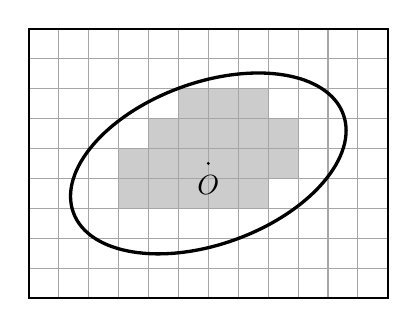
\begin{tikzpicture}[scale=0.38]
  % 填充完全在椭圆内的格子 (Ii \subset Omega)
  \foreach \x/\y in {
    3/3, 4/3, 5/3, 6/3, 7/3,
    3/4, 4/4, 5/4, 6/4, 7/4, 8/4,
    4/5, 5/5, 6/5, 7/5, 8/5,
    5/6, 6/6, 7/6
  } {
    \fill[gray!40] (\x, \y) rectangle (\x+1, \y+1);
  }
  % 网格线
  \draw[step=1, thin, gray!70] (0,0) grid (12,9);
  \draw[thick] (0,0) rectangle (12,9);
  
  % 椭圆
  \draw[very thick] (6, 4.5) ellipse [x radius=4.8, y radius=2.7, rotate=20];
  \fill (6, 4.5) circle (1.5pt) node[below=1pt] {$O$};
\end{tikzpicture}
\end{minipage}\hfill
\begin{minipage}{0.48\linewidth}
\centering
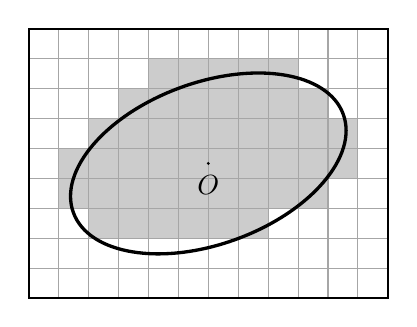
\begin{tikzpicture}[scale=0.38]
  % 填充与椭圆相交的格子 (Omega \cap Ii \neq \emptyset)
  \foreach \x/\y in {
    2/2, 3/2, 4/2, 5/2, 6/2, 7/2,
    1/3, 2/3, 3/3, 4/3, 5/3, 6/3, 7/3, 8/3, 9/3,
    1/4, 2/4, 3/4, 4/4, 5/4, 6/4, 7/4, 8/4, 9/4, 10/4,
    2/5, 3/5, 4/5, 5/5, 6/5, 7/5, 8/5, 9/5, 10/5,
    3/6, 4/6, 5/6, 6/6, 7/6, 8/6, 9/6,
    4/7, 5/7, 6/7, 7/7, 8/7
  } {
    \fill[gray!40] (\x, \y) rectangle (\x+1, \y+1);
  }
  % 网格线
  \draw[step=1, thin, gray!70] (0,0) grid (12,9);
  \draw[thick] (0,0) rectangle (12,9);
  
  % 椭圆
  \draw[very thick] (6, 4.5) ellipse [x radius=4.8, y radius=2.7, rotate=20];
  \fill (6, 4.5) circle (1.5pt) node[below=1pt] {$O$};
\end{tikzpicture}
\end{minipage}
\caption{}
\label{fig:10.2.2}
\end{figure}

\setcounter{definition}{2}
\begin{definitionp}{有面积集的等价定义}\label{def:10.2.2p}
设 $\Omega \subset \mathbb{R}^2$ 为有界集, 闭区间 $I \supset \Omega$, 对 $I$ 的分割 $T = \{I_1, I_2, \cdots, I_k\}$, 有
\[
\bigcup_{I_i\subset\Omega}I_i \subset \Omega \subset \bigcup_{\Omega\cap I_i\neq\varnothing}I_i.
\]
如果
\[
\lim_{\|T\|\to 0}\sum_{\Omega\cap I_i\neq\varnothing}v(I_i) = \lim_{\|T\|\to 0}\sum_{I_i\subset\Omega}v(I_i),
\]
则称 $\Omega$ 为有面积集, 并称 $\lim_{\|T\|\to 0}\sum_{\Omega\cap I_i\neq\varnothing}v(I_i) = \lim_{\|T\|\to 0}\sum_{I_i\subset\Omega}v(I_i)$ 为 $\Omega$ 的面积, 记为 $v(\Omega)$.
\end{definitionp}

\begin{theorem}[有面积集的几何特征二]\label{thm:10.2.5}
设 $\Omega \subset \mathbb{R}^2$ 为有界集. 则 $($图 \ref{fig:10.2.2}$)$
\[
\Omega \text{ 为有面积集} \iff \partial\Omega \text{ 为零面积集, 即 } v(\partial\Omega)=0.
\]
\end{theorem}

\begin{proof}
($\Leftarrow$) 设 $\partial\Omega$ 为零面积集, 即 $v(\partial\Omega)=0$. 又因 1 在 $\Omega$ 上连续, 故 $D_{\text{不}}^1 = \varnothing$, 当然是零面积集. 根据定理 \ref{thm:10.1.4} 知, $\partial\Omega$ 与 $D_{\text{不}}^1$ 都为零测集, 再由定理 \ref{thm:10.2.1} 推得函数 1 在 $\Omega$ 上可积, 即 $\Omega$ 为有面积集.

($\Rightarrow$) 设 $\Omega$ 为有面积集. 任取闭区间 $I \supset \Omega$, 由定理 \ref{thm:10.2.4}, $\forall\varepsilon>0$, $\exists\delta>0$, 当 $\|T\|<\delta$ 时, 有
\[
\sum_{\substack{\Omega\cap I_i\neq\varnothing \\ I_i\not\subset\Omega}}v(I_i) = \sum_{\Omega\cap I_i\neq\varnothing}v(I_i) - \sum_{I_i\subset\Omega}v(I_i) < \frac{\varepsilon}{2}.
\]
固定分割 $T=\{I_1,I_2,\cdots,I_k\}$, 显然 $\bigcup_{i=1}^{k}\partial I_i$ 为零面积集, 从而存在闭区间 $J_1,J_2,\cdots,J_s$, 使得
\[
\bigcup_{i=1}^{k}\partial I_i \subset \bigcup_{j=1}^{s}J_j, \quad \text{且} \quad \sum_{j=1}^{s}v(J_j) < \frac{\varepsilon}{2}.
\]
于是
\[
\partial\Omega \subset \left(\bigcup_{\substack{\Omega\cap I_i\neq\varnothing \\ I_i\not\subset\Omega}}I_i\right) \cup \left(\bigcup_{i=1}^{k}\partial I_i\right) \subset \left(\bigcup_{\substack{\Omega\cap I_i\neq\varnothing \\ I_i\not\subset\Omega}}I_i\right) \cup \left(\bigcup_{j=1}^{s}J_j\right),
\]
且
\[
\sum_{\substack{\Omega\cap I_i\neq\varnothing \\ I_i\not\subset\Omega}}v(I_i) + \sum_{j=1}^{s}v(J_j) < \frac{\varepsilon}{2} + \frac{\varepsilon}{2} = \varepsilon.
\]
这就证明了 $\partial\Omega$ 为零面积集. 再根据定理 \ref{thm:10.2.3}, $v(\partial\Omega)=\int_{\partial\Omega}1=0$.
\end{proof}

\begin{example}\label{ex:10.2.2}
由定理 \ref{thm:10.1.4} 中反例知, $\mathbb{Q}^2 \cap [0,1]^2$ 为 $\mathbb{R}^2$ 中的有界非零面积集. 再由 $v(\partial(\mathbb{Q}^2 \cap [0,1]^2)) = v([0,1]^2) = 1 \neq 0$ 及定理 \ref{thm:10.2.5} 推得 $\mathbb{Q}^2 \cap [0,1]^2$ 不为有面积集. 根据定义 \ref{def:10.2.2}, 1 在 $\Omega$ 上不可积.
\end{example}

\setcounter{definition}{2}
\begin{definitionpp}{有面积集的等价定义}\label{def:10.2.2pp}
设 $\Omega \subset \mathbb{R}^2$ 为有界集. 如果 $\partial\Omega$ 为零面积集, 则称 $\Omega$ 为有面积集.
\end{definitionpp}

因为有时对 $\partial\Omega$ 是否为零面积集的判断比较容易, 所以用这种方法判断 $\Omega$ 是否为有面积集也比较容易. 但是, 这定义不能给出 $\Omega$ 的面积的大小.

\begin{theorem}[有面积集上函数可积的充要条件]\label{thm:10.2.6}
设 $\Omega \subset \mathbb{R}^2$ 为有面积集, $f\colon \Omega \to \mathbb{R}$ 为有界二元函数. 则
\begin{align*}
f \text{ 在 } \Omega \text{ 上可积} &\iff D_{\text{不}}^f = \{(x, y) \in \Omega \mid f \text{ 在 } (x, y) \text{ 处不连续}\} \text{ 为零测集}, \\
&\quad\text{即 } f \text{ 在 } \Omega \text{ 上几乎处处连续}.
\end{align*}
\end{theorem}

\begin{proof}
因为 $\Omega$ 为有面积集, 根据定理 \ref{thm:10.2.5} 知, $\partial\Omega$ 与 $\partial\Omega\cap\Omega$ 都为零面积集, 当然它们也为零测集.

设闭区间 $I \supset \Omega$, 则 $\Omega = \Omega^\circ \cup (\partial \Omega \cap \Omega)$, 且
\[
I = \Omega^\circ \cup \partial\Omega \cup (I\setminus\Omega)^\circ \cup \partial I.
\]
显然, $\partial I$ 为零面积集, 自然也为零测集. 此外, 易见,
\begin{gather*}
f \text{ 在 } \boldsymbol{x} \in \Omega \text{ 不连续} \implies f_{\Omega} \text{ 在 } \boldsymbol{x} \in \Omega \text{ 不连续}; \\
f \text{ 在 } \boldsymbol{x} \in \Omega^\circ \text{ 不连续} \iff f_{\Omega} \text{ 在 } \boldsymbol{x} \in \Omega^\circ \text{ 不连续};
\end{gather*}
$f_{\Omega}$ 在 $(I\setminus\Omega)^\circ$ 上恒为 0, 故它连续.
于是
\[
\begin{cases}
D_{\text{不}}^f \subset D_{\text{不}}^{f_{\Omega}}, \\
D_{\text{不}}^{f_{\Omega}} \subset D_{\text{不}}^f \cup \partial\Omega \cup \partial I.
\end{cases}
\]
这就可推出
\begin{align*}
f \text{ 在 } \Omega \text{ 上可积} &\iff f_{\Omega} \text{ 在 } I \text{ 上可积} \iff D_{\text{不}}^{f_{\Omega}} \text{ 为零测集} \\
&\iff D_{\text{不}}^f \text{ 为零测集, 即 } f \text{ 在 } \Omega \text{ 上几乎处处连续}. \qedhere
\end{align*}
\end{proof}

注意, 0 在任何有界集 $\Omega \subset \mathbb{R}^2$ 上都可积, 不必要求 $\Omega$ 为有面积集. 而定理 \ref{thm:10.2.6} 是在 $\Omega$ 为有面积集的前提下 $f$ 可积的充要条件. 定义 \ref{def:10.2.2} 表明 1 在 $\Omega$ 上可积就是 $\Omega$ 为有面积集.

\begin{example}\label{ex:10.2.3}
设 $\Omega$ 为有限段显式表示的连续曲线围成的区域 (图 \ref{fig:10.2.3}), 根据例 \ref{ex:10.1.1} 知 $\partial\Omega$ 为零面积集, 即 $v(\partial\Omega)=0$. 再根据定理 \ref{thm:10.2.5}, $\Omega$ 为有面积集.

同理, 若 $\Omega$ 为有限段 $C^1$ 参数曲线围成的区域 (图 \ref{fig:10.2.4}), 根据例 \ref{ex:10.1.2} 知, $\partial\Omega$ 为零面积集. 再由定理 \ref{thm:10.2.5}, $\Omega$ 为有面积集.
\end{example}

\begin{figure}[htbp]
\centering
\begin{minipage}{0.48\linewidth}
\centering
\begin{tikzpicture}[scale=0.9, >=Stealth]
  % 坐标轴
  \draw[->] (-0.3, 0) -- (4.2, 0) node[below] {$x$};
  \draw[->] (0, -0.3) -- (0, 3.6) node[left] {$y$};
  \node[below left] at (0,0) {$O$};
  
  % 区域四条曲线:
  \begin{scope}
    \path[clip] (0.5, 0.9) to[bend right=10] (1.1, 0.5)
                           to[bend right=12] (3.0, 0.9)
                           to[bend left=10] (2.3, 2.3)
                           to[bend left=15] (0.5, 0.9);
    \fill[pattern=north east lines, pattern color=black!70] (0,0) rectangle (4,4);
  \end{scope}
  \draw[thick] (0.5, 0.9) to[bend right=10] (1.1, 0.5)
                          to[bend right=12] (3.0, 0.9)
                          to[bend left=10] (2.3, 2.3)
                          to[bend left=15] (0.5, 0.9);
  \node at (1.8, 1.3) {$\Omega$};
  
  % 曲线标注
  \node[left, rotate=38] at (0.7, 0.6) {\scriptsize $x=g_1(y)$};
  \node[below] at (2.0, 0.65) {\scriptsize $y=f_1(x)$};
  \node[right, rotate=-55] at (2.7, 1.7) {\scriptsize $x=g_2(y)$};
  \node[above, rotate=38] at (1.3, 1.8) {\scriptsize $y=f_2(x)$};
\end{tikzpicture}
\caption{}
\label{fig:10.2.3}
\end{minipage}\hfill
\begin{minipage}{0.48\linewidth}
\centering
\begin{tikzpicture}[scale=0.9, >=Stealth]
  % 坐标轴
  \draw[->] (-0.3, 0) -- (4.2, 0) node[below] {$x$};
  \draw[->] (0, -0.3) -- (0, 3.6) node[left] {$y$};
  \node[below left] at (0,0) {$O$};
  
  % 梅花状参数曲线
  \begin{scope}
    \path[clip] (2.0, 0.5) to[out=20, in=200] (2.8, 0.6)
                           to[out=60, in=-40] (2.6, 1.4)
                           to[out=0, in=-90] (3.3, 2.0)
                           to[out=90, in=0] (2.5, 2.6)
                           to[out=140, in=40] (1.5, 2.6)
                           to[out=180, in=90] (0.7, 2.0)
                           to[out=-90, in=180] (1.4, 1.4)
                           to[out=-140, in=120] (1.2, 0.6)
                           to[out=-20, in=160] (2.0, 0.5);
    \fill[pattern=north east lines, pattern color=black!70] (0,0) rectangle (4,4);
  \end{scope}
  \draw[thick] (2.0, 0.5) to[out=20, in=200] (2.8, 0.6)
                          to[out=60, in=-40] (2.6, 1.4)
                          to[out=0, in=-90] (3.3, 2.0)
                          to[out=90, in=0] (2.5, 2.6)
                          to[out=140, in=40] (1.5, 2.6)
                          to[out=180, in=90] (0.7, 2.0)
                          to[out=-90, in=180] (1.4, 1.4)
                          to[out=-140, in=120] (1.2, 0.6)
                          to[out=-20, in=160] (2.0, 0.5);
  \node at (2.0, 1.7) {$\Omega$};
  \node[right] at (3.3, 2.0) {\small $(x(t), y(t))$};
\end{tikzpicture}
\caption{}
\label{fig:10.2.4}
\end{minipage}
\end{figure}

上面所述的区域 $\Omega$ 是数学分析中常见的集合. 再从定理 \ref{thm:10.2.6} 立即得到
\[
f\colon\Omega\to\mathbb{R} \text{ 可积} \iff f \text{ 在 } \Omega \text{ 上几乎处处连续}.
\]

最后, 我们来讨论可积函数的一些性质.

\begin{theorem}\label{thm:10.2.7}
设 $\Omega \subset \mathbb{R}^2$ 为有界集, $f, f_1, f_2\colon \Omega \to \mathbb{R}$ 都为二元函数, $c \in \mathbb{R}$ 为常数.
\begin{enumerate}
\item 如果 $\Omega$ 为有面积集, 则 $c$ 在 $\Omega$ 上可积, 且
\[
\int_{\Omega}c = c v(\Omega).
\]
\item 如果 $f$ 在 $\Omega$ 上可积, 则 $cf$ 在 $\Omega$ 上也可积, 且
\[
\int_{\Omega}cf = c\int_{\Omega}f.
\]
\item 如果 $f_{1}$ 与 $f_{2}$ 都在 $\Omega$ 上可积, 则 $f_{1} + f_{2}$ 在 $\Omega$ 上也可积, 且
\[
\int_{\Omega}(f_{1}+f_{2}) = \int_{\Omega}f_{1} + \int_{\Omega}f_{2}.
\]
\item 如果 $f$ 在 $\Omega$ 上可积, 且 $f \geqslant 0$, 则
\[
\int_{\Omega}f \geqslant 0;
\]
特别地, 若 $f_{1}$ 与 $f_{2}$ 都在 $\Omega$ 上可积, 且 $f_{1} \geqslant f_{2}$, 则
\[
\int_{\Omega}f_{1} \geqslant \int_{\Omega}f_{2}.
\]
\item 如果 $f$ 在 $\Omega$ 上可积, 则 $|f|$ 在 $\Omega$ 上也可积, 且
\[
\left|\int_{\Omega}f\right| \leqslant \int_{\Omega}|f|.
\]
\end{enumerate}
\end{theorem}

\begin{proof}
设 $I \subset \mathbb{R}^2$ 为闭区间, 且 $I \supset \Omega$. 先证 (2), 再证 (1).

(2) $\int_{\Omega} cf = \int_{I}(cf)_{\Omega} = \int_{I} cf_{\Omega} = c\int_{I} f_{\Omega} = c\int_{\Omega} f$.

(1) 因为 $\Omega$ 为有面积集, 由 (2) 知 $c = c \cdot 1$ 在 $\Omega$ 上也可积, 且
\[
\int_{\Omega}c = \int_{\Omega}c \cdot 1 = c\int_{\Omega}1 = c v(\Omega).
\]

(3) 因为 $f_{1}$ 与 $f_{2}$ 都在 $\Omega$ 上可积, 故 $f_{1\Omega}$ 与 $f_{2\Omega}$ 都在 $I$ 上可积, 从而 $(f_{1}+f_{2})_{\Omega}=f_{1\Omega}+f_{2\Omega}$ 也在 $I$ 上可积, 即 $f_{1}+f_{2}$ 在 $\Omega$ 上可积, 且
\[
\int_{\Omega}(f_{1}+f_{2}) = \int_{I}(f_{1}+f_{2})_{\Omega} = \int_{I}(f_{1\Omega}+f_{2\Omega}) = \int_{I}f_{1\Omega} + \int_{I}f_{2\Omega} = \int_{\Omega}f_{1} + \int_{\Omega}f_{2}.
\]

(4) 因为在 $\Omega$ 上 $f \geqslant 0$, 所以 $f_{\Omega} \geqslant 0$. 根据定理 \ref{thm:10.1.1}(4), 有
\[
\int_{\Omega}f = \int_{I}f_{\Omega} \geqslant 0.
\]
从而
\[
\int_{\Omega}f_{1} - \int_{\Omega}f_{2} = \int_{\Omega}(f_{1}-f_{2}) \geqslant 0,
\]
\[
\int_{\Omega}f_{1} \geqslant \int_{\Omega}f_{2}.
\]

(5) 因为 $f$ 在 $\Omega$ 上可积, 所以 $f_{\Omega}$ 在 $I$ 上可积, 从而 $|f|_{\Omega}=|f_{\Omega}|$ 在 $I$ 上可积. 再由
\[
-|f| \leqslant f \leqslant |f|
\]
及 (4) 得到
\begin{gather*}
-\int_{\Omega}|f| \leqslant \int_{\Omega}f \leqslant \int_{\Omega}|f|, \\
\left|\int_{\Omega}f\right| \leqslant \int_{\Omega}|f|. \qedhere
\end{gather*}
\end{proof}

\begin{theorem}[积分的集合可加性]\label{thm:10.2.8}
设 $\Omega_{1}, \Omega_{2} \subset \mathbb{R}^{2}$ 都为有界集, 且 $\Omega_{1} \cap \Omega_{2}$ 为一零面积集 $(\Omega_{1} \cap \Omega_2 = \varnothing$ 为其特例$)$. 若函数 $f$ 在 $\Omega_{1}$ 与 $\Omega_{2}$ 上都可积, 则 $f$ 在 $\Omega_{1} \cup \Omega_{2}$ 上也可积, 且
\[
\int_{\Omega_{1}\cup\Omega_{2}}f = \int_{\Omega_{1}}f + \int_{\Omega_{2}}f.
\]
\end{theorem}

\begin{proof}
显然, 除了一个零面积集, 成立等式 $f_{\Omega_1 \cup \Omega_2} = f_{\Omega_1} + f_{\Omega_2}$. 设闭区间 $I \supset \Omega_1 \cup \Omega_2$, 则有
\[
\int_{\Omega_{1}}f + \int_{\Omega_{2}}f = \int_{I}f_{\Omega_{1}} + \int_{I}f_{\Omega_{2}} = \int_{I}(f_{\Omega_{1}}+f_{\Omega_{2}}) \reason{\text{例 \ref{ex:10.1.5}}} \int_{I}f_{\Omega_{1}\cup\Omega_{2}} = \int_{\Omega_{1}\cup\Omega_{2}}f. \qedhere
\]
\end{proof}

\begin{theorem}[积分中值定理]\label{thm:10.2.9}
设 $\Omega \subset \mathbb{R}^2$ 为有面积的连通紧致集, $f, g\colon \Omega \to \mathbb{R}$ 连续, 且 $g$ 在 $\Omega$ 上不变号, 则 $\exists\boldsymbol{\xi} \in \Omega$, s.t.
\[
\int_{\Omega}f g = f(\boldsymbol{\xi})\int_{\Omega}g.
\]
特别地, 取 $g=1$, 则 $\exists\boldsymbol{\xi} \in \Omega$, s.t.
\[
\int_{\Omega}f = f(\boldsymbol{\xi})v(\Omega).
\]
\end{theorem}

\begin{proof}
因为 $\Omega$ 为有面积集, 根据定理 \ref{thm:10.2.5}, $v(\partial\Omega)=0$ (即 $\partial\Omega$ 为零面积集). 由于 $f, g$ 在 $\Omega$ 上连续, 故 $fg$ 在 $\Omega$ 上也连续. 再根据定理 \ref{thm:10.2.1} 或定理 \ref{thm:10.2.6}, $g$ 与 $fg$ 都在 $\Omega$ 上可积. 又因 $\Omega$ 紧致, 故连续函数 $f$ 在 $\Omega$ 上达到最大值与最小值, 所以 $\exists\boldsymbol{p}, \boldsymbol{q} \in \Omega$, s.t.
\[
f(\boldsymbol{p}) = \max f(\Omega), \quad f(\boldsymbol{q}) = \min f(\Omega).
\]
从题设 $g$ 在 $\Omega$ 上不变号, 不妨设 $g|_{\Omega} \geqslant 0$. 于是
\[
f(\boldsymbol{q})g \leqslant fg \leqslant f(\boldsymbol{p})g.
\]
根据定理 \ref{thm:10.2.7}(4), (2), 有
\[
f(\boldsymbol{q})\int_{\Omega}g \leqslant \int_{\Omega}fg \leqslant f(\boldsymbol{p})\int_{\Omega}g.
\]
(1) 若 $\int_{\Omega}g=0$, 由 $g$ 非负连续, $g|_{\Omega}\equiv 0$, 则 $\int_{\Omega}fg=0=f(\boldsymbol{\xi})\cdot 0=f(\boldsymbol{\xi})\int_{\Omega}g$, $\forall\boldsymbol{\xi}\in\Omega$.

(2) 若 $\int_{\Omega}g\neq 0$, 由 $g\geqslant 0$ 知 $\int_{\Omega}g>0$. 于是
\[
f(\boldsymbol{q}) \leqslant \frac{\displaystyle\int_{\Omega}fg}{\displaystyle\int_{\Omega}g} \leqslant f(\boldsymbol{p}).
\]
再由 $\Omega$ 连通, 应用连续函数的介值定理, $\exists\boldsymbol{\xi}\in\Omega$, s.t.
\[
\frac{\displaystyle\int_{\Omega}fg}{\displaystyle\int_{\Omega}g} = f(\boldsymbol{\xi}),
\]
即
\[
\int_{\Omega}fg = f(\boldsymbol{\xi})\int_{\Omega}g. \qedhere
\]
\end{proof}

\begin{exblock}{练习题 10.2}
1. 设 $f$ 为连续函数, 求极限
\[
\lim_{r \to 0}\frac{1}{\pi r^2}\iint_{x^2 + y^2 \leqslant r^2} f(x, y)\,\mathrm{d}x\mathrm{d}y.
\]

2. 证明:
\[
1.96 < \iint_{|x|+|y|\leqslant 10}\frac{\mathrm{d}x\mathrm{d}y}{100 + \cos^2 x + \cos^2 y} < 2.
\]
\end{exblock}
